% =============================================================================
% cs-pipeline-timing.tex — Instruction pipeline timing diagram (5-stage)
%
% Shows: four instructions flowing through IF/ID/EX/MEM/WB across nine clock
% cycles, with the diagonal "staircase" that makes pipelining legible, plus a
% marked stall.
% Compiles standalone via: xelatex cs-pipeline-timing.tex
%
% Use for: computer organization (pipelining, hazards, speedup), computer
% architecture (CPI, throughput vs. latency).
%
% To show a HAZARD: shift one instruction's remaining stages one column right
% and put a shaded "stall" cell in the gap (as done for I3 below).
% =============================================================================

\documentclass[border=5pt]{standalone}
\usepackage{tikz}
\usetikzlibrary{arrows.meta, positioning}

\definecolor{stage-border}{HTML}{012169}
\definecolor{stage-fill}{HTML}{E8EDF5}
\definecolor{stall-fill}{HTML}{FBE3E3}
\definecolor{stall-border}{HTML}{B91C1C}
\definecolor{header}{HTML}{012169}
\definecolor{muted}{HTML}{525252}

\tikzset{
  stage/.style={
    draw=stage-border, fill=stage-fill, thick,
    minimum width=1.15cm, minimum height=0.75cm, align=center, font=\scriptsize
  },
  stall/.style={
    draw=stall-border, fill=stall-fill, thick, dashed,
    minimum width=1.15cm, minimum height=0.75cm, align=center,
    font=\scriptsize, text=stall-border
  },
  chead/.style={font=\scriptsize\bfseries, text=header},
  rowlbl/.style={font=\small\bfseries, text=header},
  note/.style={font=\scriptsize, text=muted}
}

% -----------------------------------------------------------------------------
% Diagram: 5-stage pipeline, 4 instructions, 9 cycles.
% Grid: cell (cycle c, instruction r) sits at
%   x = 1.2*c ,  y = -0.85*r     for c = 1..9, r = 1..4
% Cycle headers sit at y = 0.75 (one full cell-height above row 1's centre at
% y = -0.85, so 0.85+0.375 = 1.225cm of clearance to the box top — no overlap).
% Instruction labels sit at x = -0.35, left of column 1 (x = 1.2, half-width
% 0.575 -> left edge 0.625), giving 0.99cm of clear margin (P7c).
% I3 stalls one cycle in EX: its MEM/WB shift right by one column and a dashed
% stall cell fills the gap at cycle 6.
% -----------------------------------------------------------------------------

\begin{document}
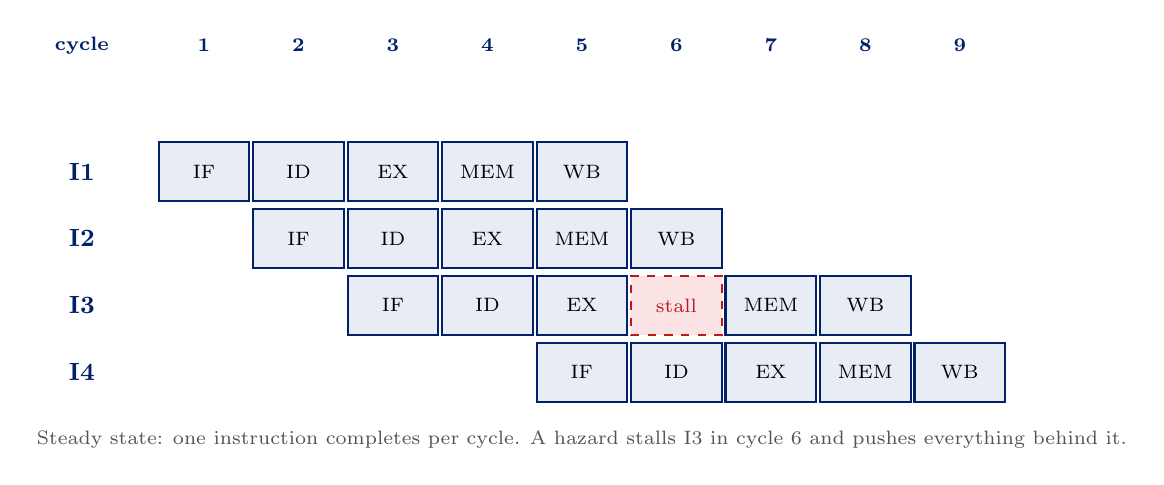
\begin{tikzpicture}

  % ---- Cycle headers -------------------------------------------------------
  \foreach \c in {1,...,9} {
    \node[chead] at (1.2*\c, 0.75) {\c};
  }
  \node[chead] at (-0.35, 0.75) {cycle};

  % ---- I1: IF ID EX MEM WB  (cycles 1-5) ----------------------------------
  \node[rowlbl] at (-0.35, -0.85) {I1};
  \foreach \s [count=\c from 1] in {IF, ID, EX, MEM, WB} {
    \node[stage] at (1.2*\c, -0.85) {\s};
  }

  % ---- I2: cycles 2-6 ------------------------------------------------------
  \node[rowlbl] at (-0.35, -1.70) {I2};
  \foreach \s [count=\i from 0] in {IF, ID, EX, MEM, WB} {
    \pgfmathtruncatemacro{\c}{\i + 2}
    \node[stage] at (1.2*\c, -1.70) {\s};
  }

  % ---- I3: cycles 3-5, STALL at 6, then MEM/WB at 7-8 ---------------------
  \node[rowlbl] at (-0.35, -2.55) {I3};
  \foreach \s [count=\i from 0] in {IF, ID, EX} {
    \pgfmathtruncatemacro{\c}{\i + 3}
    \node[stage] at (1.2*\c, -2.55) {\s};
  }
  \node[stall] at (1.2*6, -2.55) {stall};
  \node[stage] at (1.2*7, -2.55) {MEM};
  \node[stage] at (1.2*8, -2.55) {WB};

  % ---- I4: delayed behind the stall, cycles 5-9 ---------------------------
  \node[rowlbl] at (-0.35, -3.40) {I4};
  \foreach \s [count=\i from 0] in {IF, ID, EX, MEM, WB} {
    \pgfmathtruncatemacro{\c}{\i + 5}
    \node[stage] at (1.2*\c, -3.40) {\s};
  }

  % ---- Caption -------------------------------------------------------------
  \node[note, align=center] at (6.0, -4.25)
        {Steady state: one instruction completes per cycle.
         A hazard stalls I3 in cycle 6 and pushes everything behind it.};

\end{tikzpicture}
\end{document}
